\documentclass{article}

\usepackage{Sweave}
\begin{document}
\Sconcordance{concordance:tidigg.tex:tidigg.Rnw:%
1 2 1 1 0 2 1 1 2 1 0 3 1 1 2 4 0 1 3 5 0 1 3 5 0 1 3 5 0 1 9 7 0 1 4 7 %
0 1 2 1 5 8 0 1 10 12 0 1 4 6 0 1 2 1 1 1 3 6 0 1 4 6 0 2 2 5 0 1 3 5 0 %
2 2 5 0 1 5 7 0 1 3 1 0 3 1 1 2 2 1 3 0 2 2 5 0 1 4 6 0 1 4 6 0 2 2 19 %
0 1 1 22 0 1 3 2 1 1 2 27 0 1 1 6 0 1 1 7 0 1 3 4 0 1 2 2 1}


\begin{Schunk}
\begin{Sinput}
> library(tidyverse)
> library(readxl)
>     raclav19 <- read_excel("~/Scrivania/Trasfusionale/datiprover/raclav19.xls")
> raclav19ce <- filter(raclav19, cod_emc=="25")
> # select per colonne; filter per righe. 
> scarico19 <- read_excel("~/Scrivania/Trasfusionale/datiprover/scarico19.xls")
\end{Sinput}
\end{Schunk}
\begin{Schunk}
\begin{Sinput}
> ggplot(data = diamonds) + geom_bar(mapping = aes(x = cut))
\end{Sinput}
\end{Schunk}
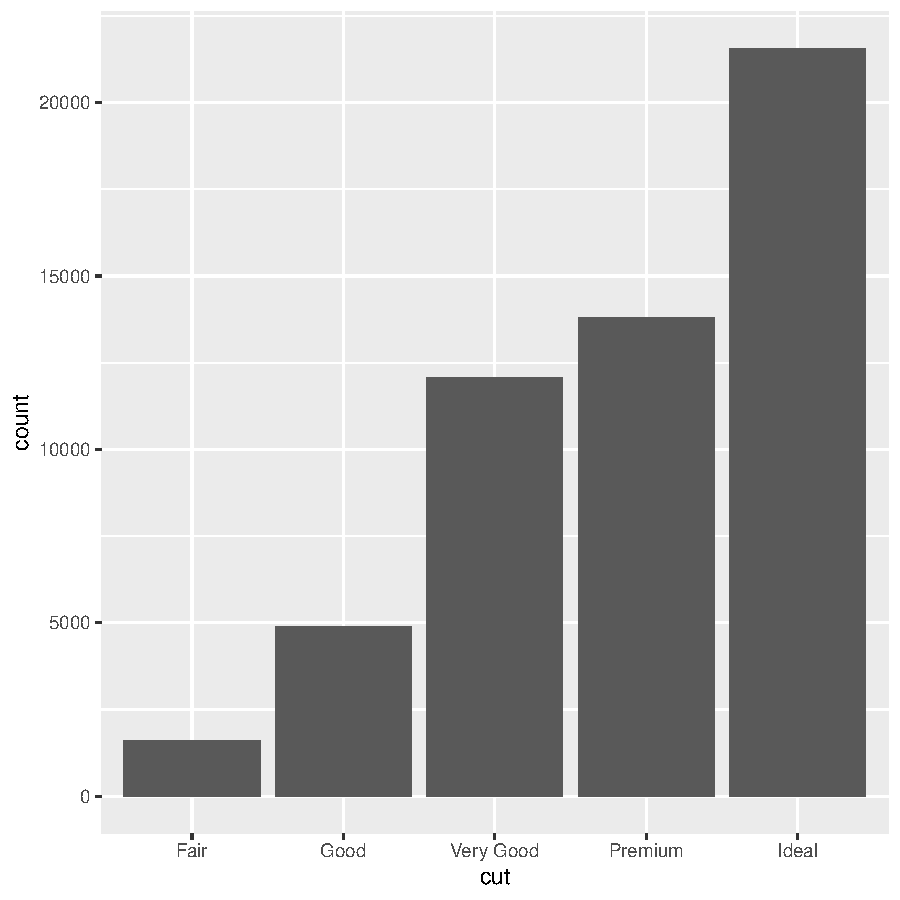
\includegraphics{tidigg-002}
\begin{Schunk}
\begin{Sinput}
> ggplot(data = diamonds) + stat_count(mapping = aes(x = cut))
\end{Sinput}
\end{Schunk}
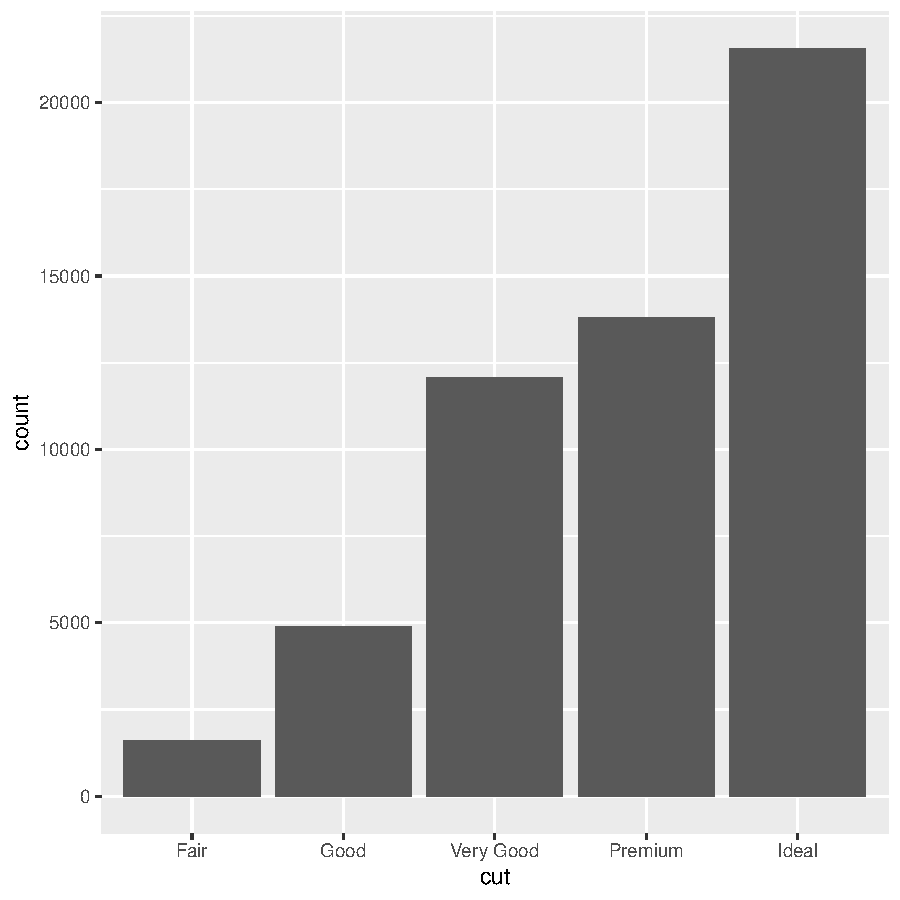
\includegraphics{tidigg-003}
\begin{Schunk}
\begin{Sinput}
> ggplot(data = diamonds) + stat_density(mapping = aes(x = cut))
\end{Sinput}
\end{Schunk}
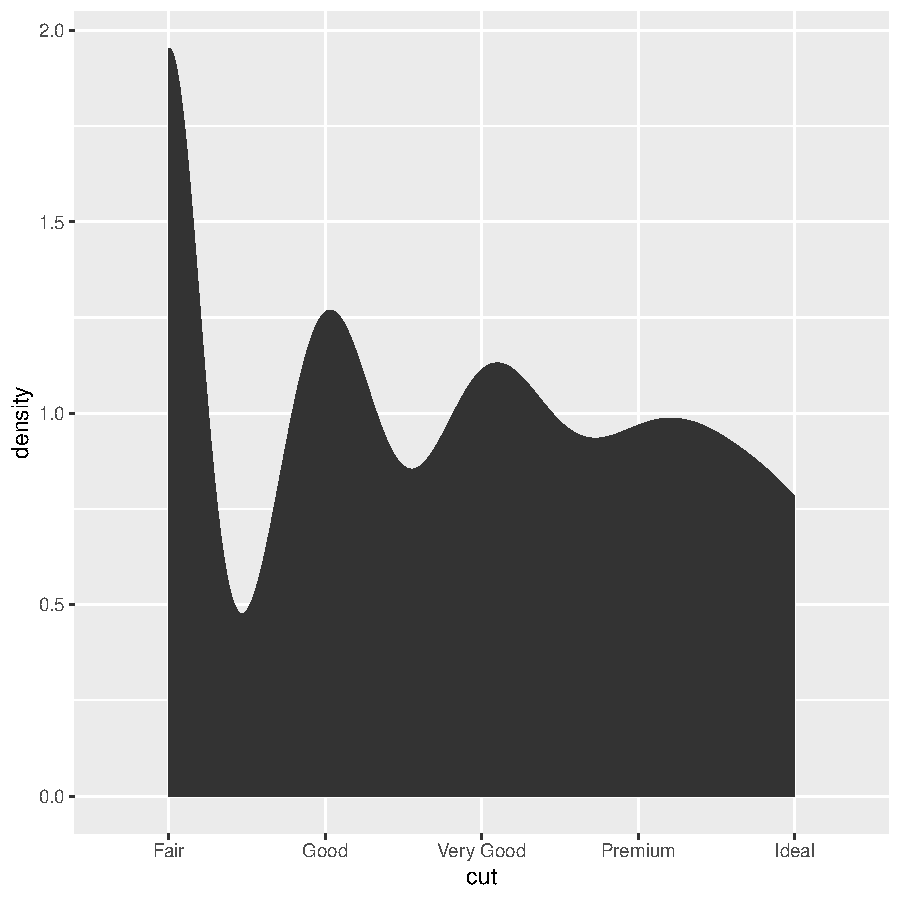
\includegraphics{tidigg-004}
\begin{Schunk}
\begin{Sinput}
> demo <- tribble(
+ ~a,
+ ~b,
+ "bar_1", 20,
+ "bar_2", 30,
+ "bar_3", 40
+ )
> ggplot(data = demo) +
+ geom_bar(
+ mapping = aes(x = a, y = b), stat = "identity"
+ )
\end{Sinput}
\end{Schunk}
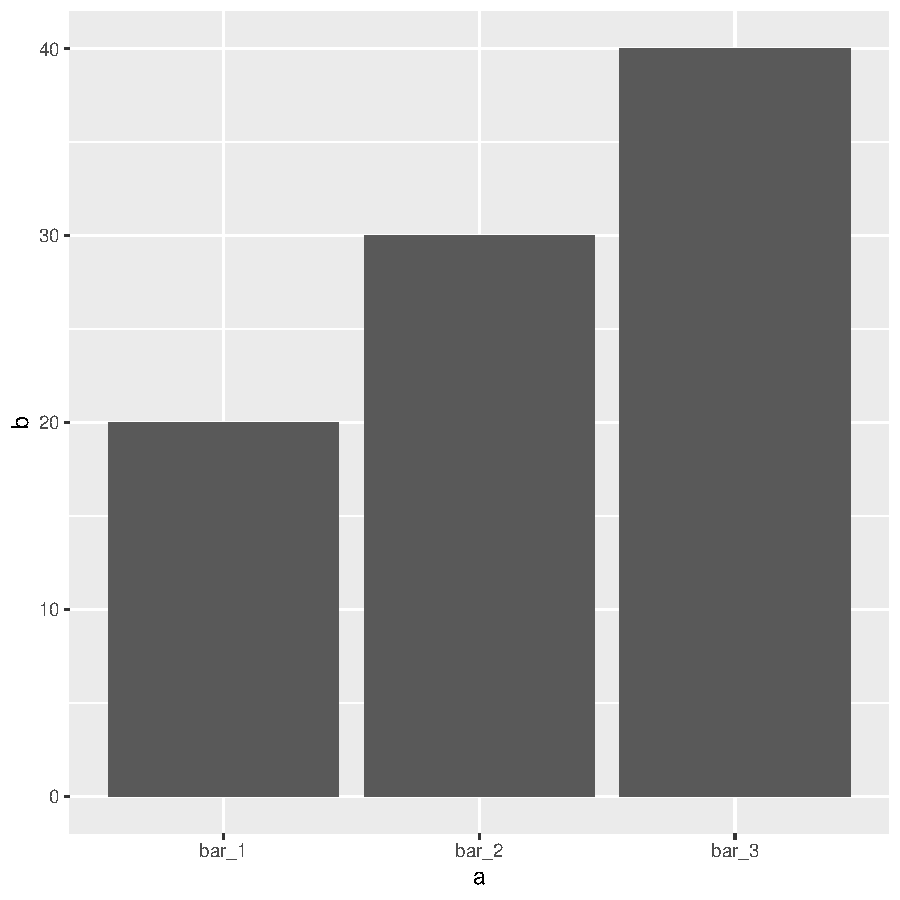
\includegraphics{tidigg-005}

\begin{Schunk}
\begin{Sinput}
> # In Percentuale proporzione
> ggplot(data = diamonds) +
+ geom_bar(
+ mapping = aes(x = cut, y = ..prop.., group = 1))
\end{Sinput}
\end{Schunk}
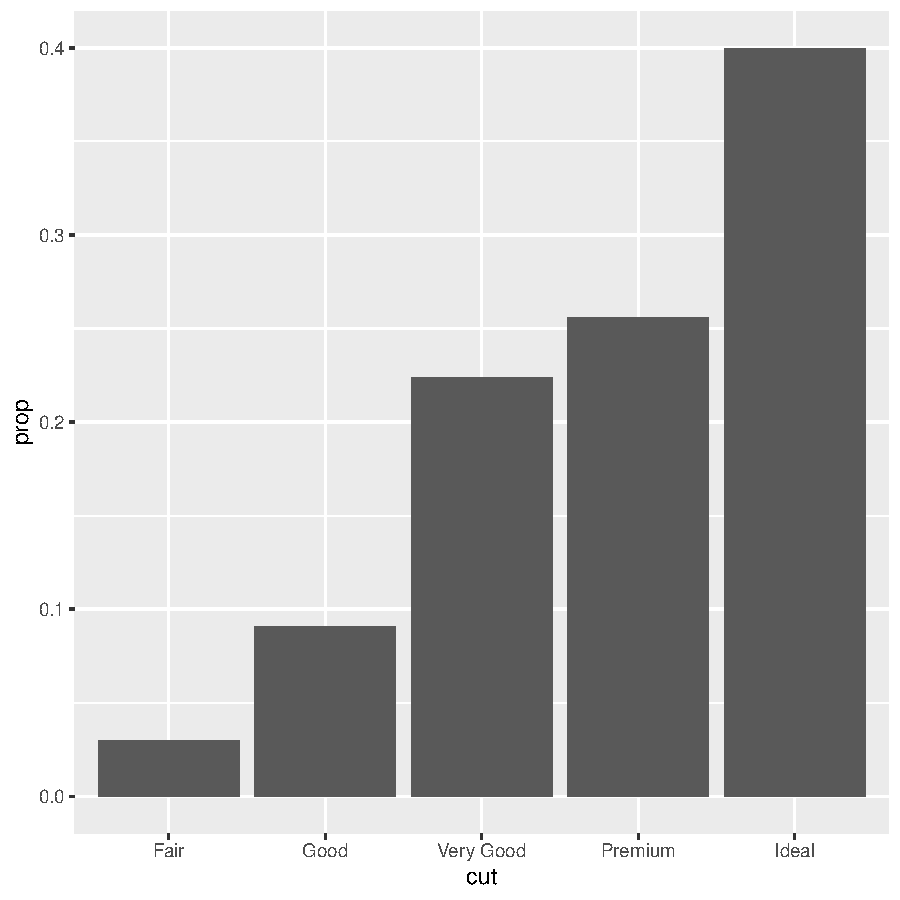
\includegraphics{tidigg-006}
\begin{Schunk}
\begin{Sinput}
> ggplot(data = diamonds) +
+ stat_summary(
+ mapping = aes(x = cut, y = depth),
+ fun.ymin = min,
+ fun.ymax = max,
+ fun.y = median
+ 
+ )
\end{Sinput}
\end{Schunk}
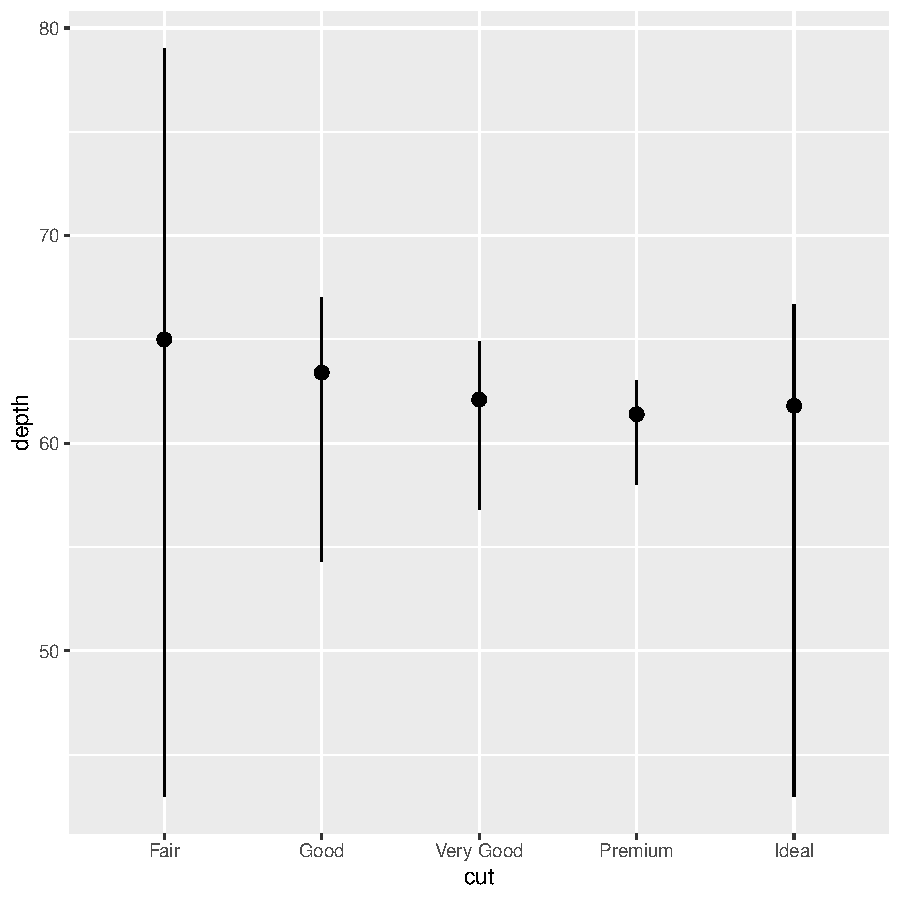
\includegraphics{tidigg-007}
\begin{Schunk}
\begin{Sinput}
> ggplot(data = diamonds) +
+ geom_bar(mapping = aes(x = cut, color = cut))
\end{Sinput}
\end{Schunk}
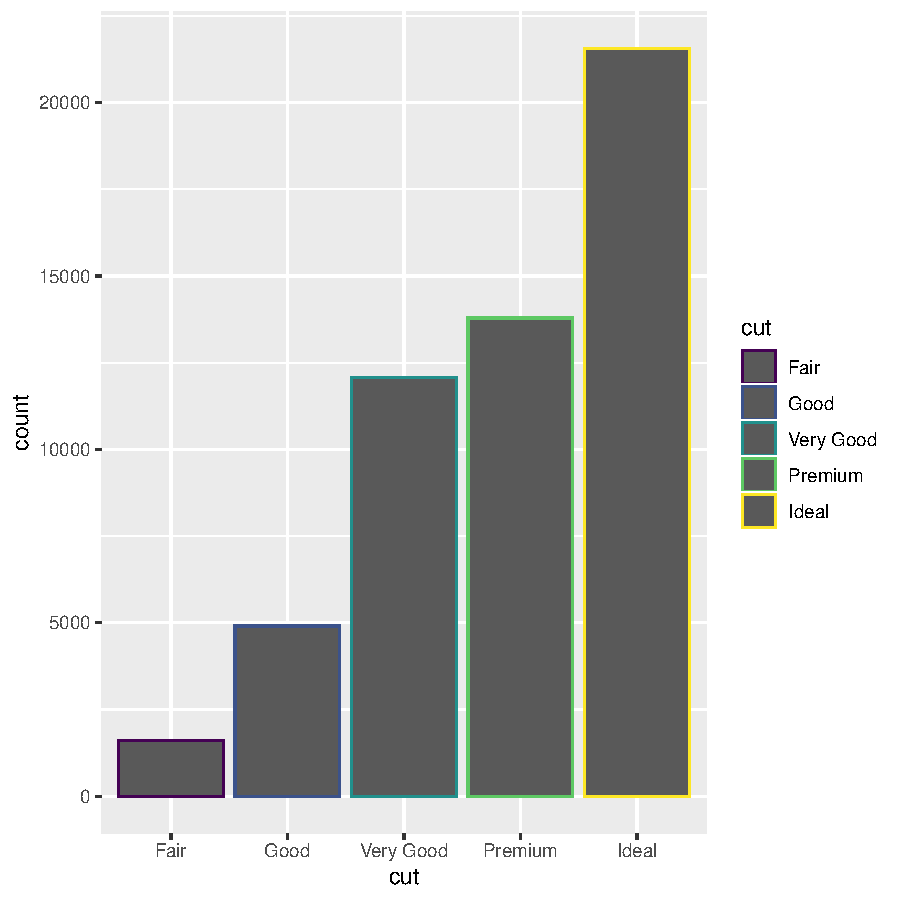
\includegraphics{tidigg-008}


\begin{Schunk}
\begin{Sinput}
> ggplot(data = diamonds) +
+ geom_bar(mapping = aes(x = cut, fill = cut))
\end{Sinput}
\end{Schunk}
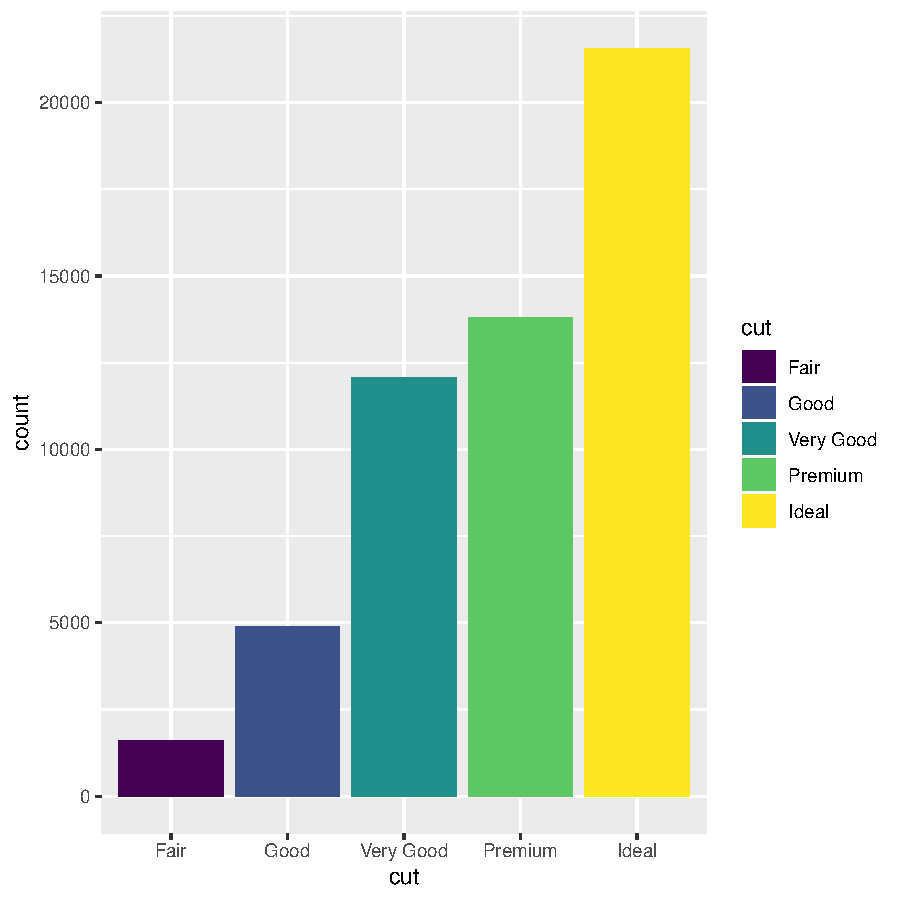
\includegraphics{tidigg-009}
\begin{Schunk}
\begin{Sinput}
> ggplot(data = diamonds) +
+ geom_bar(mapping = aes(x = cut, fill = clarity))
\end{Sinput}
\end{Schunk}
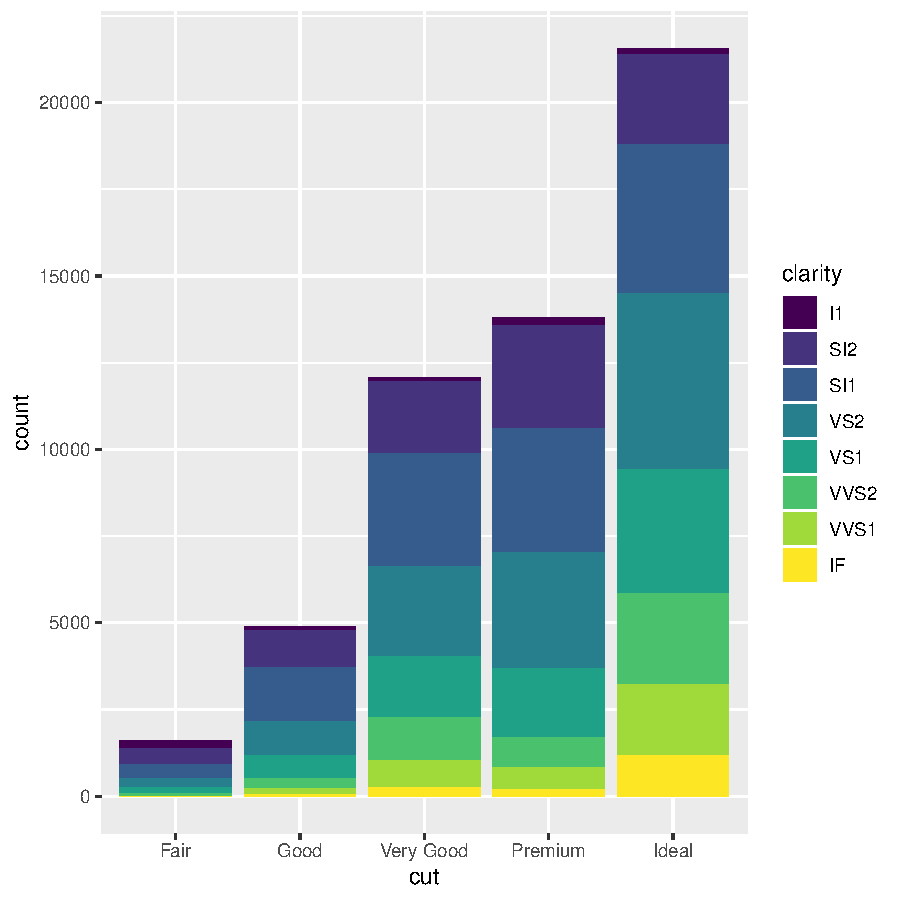
\includegraphics{tidigg-010}

\begin{Schunk}
\begin{Sinput}
> ggplot(data = diamonds) + geom_bar(mapping = aes(x = cut, fill = clarity))
\end{Sinput}
\end{Schunk}
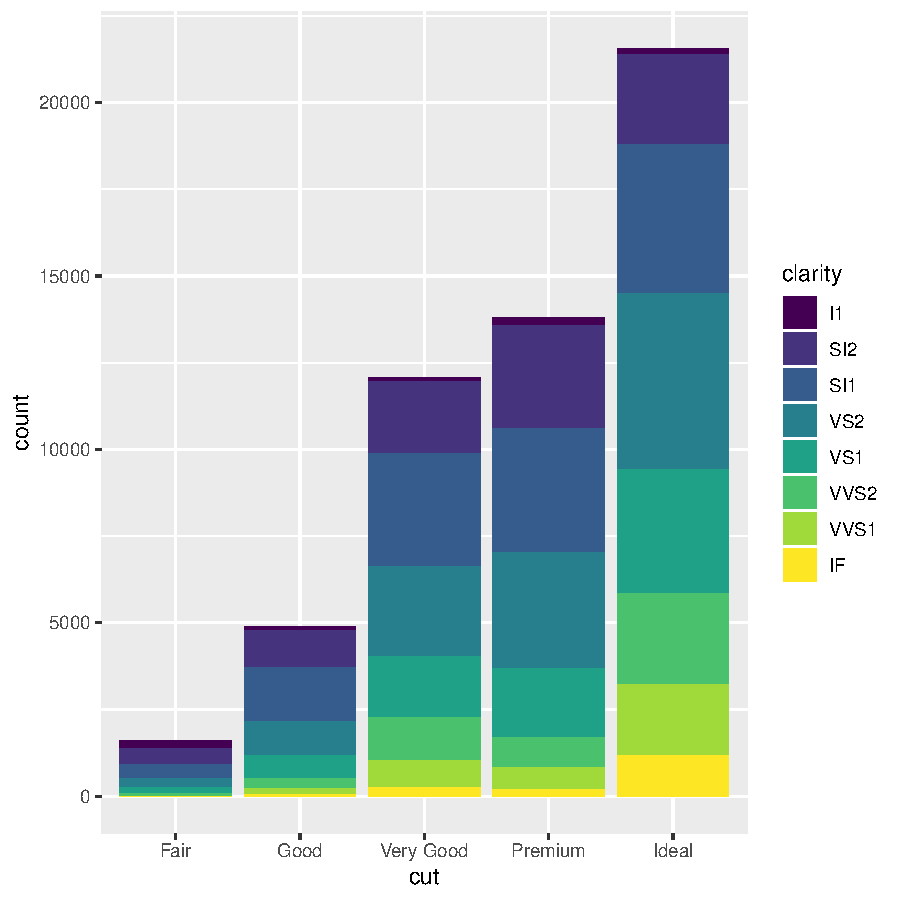
\includegraphics{tidigg-011}
\begin{Schunk}
\begin{Sinput}
> ggplot(data = diamonds) + geom_bar(mapping = aes(x = cut, fill = clarity), position = "fill")
\end{Sinput}
\end{Schunk}
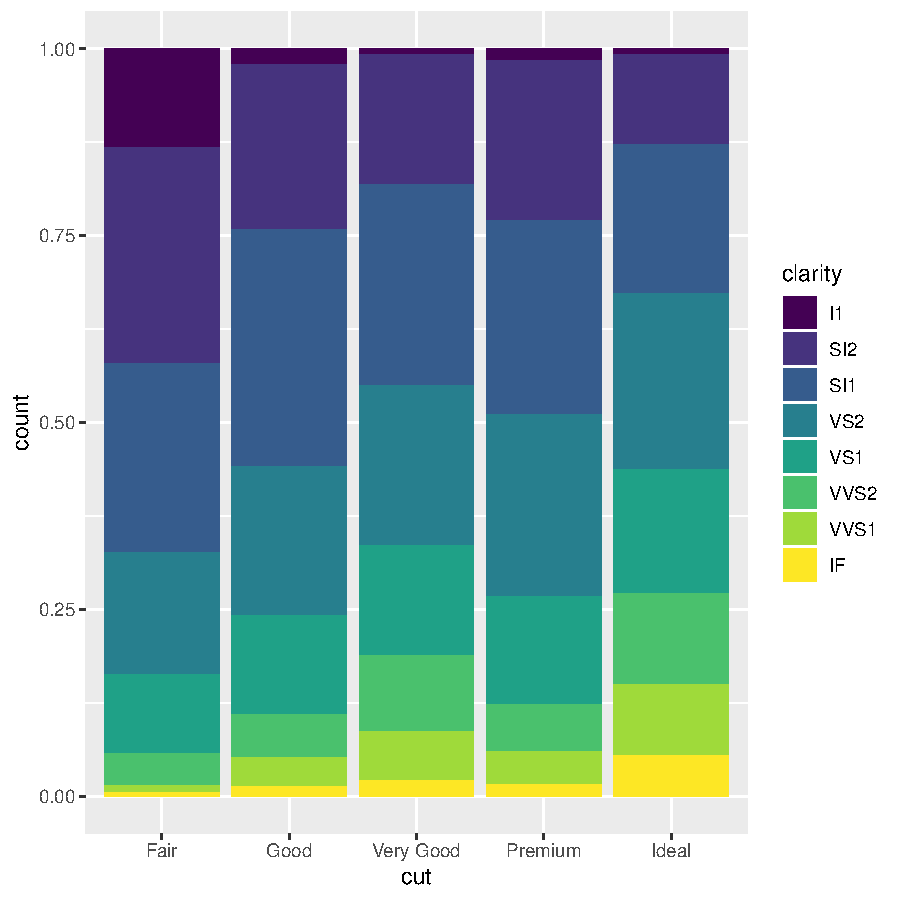
\includegraphics{tidigg-012}

\begin{Schunk}
\begin{Sinput}
> ggplot(data = raclav19ce) + geom_bar(mapping = aes(x = tipo_sacca, fill = lotto))
\end{Sinput}
\end{Schunk}
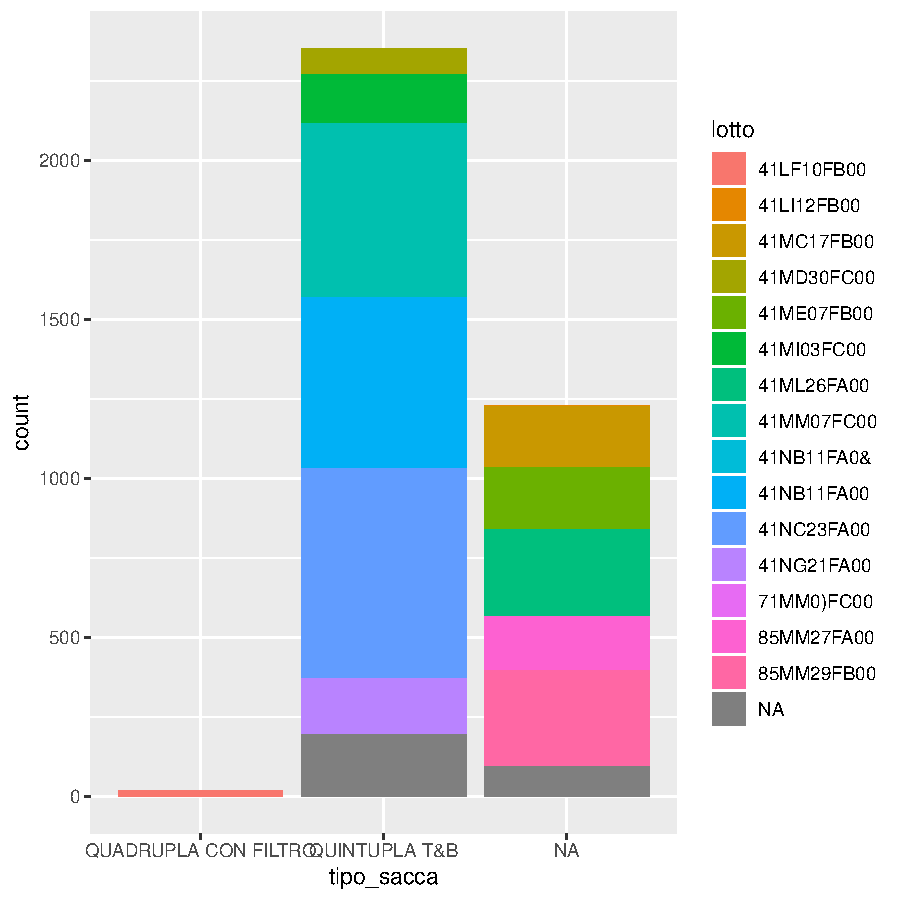
\includegraphics{tidigg-013}
\begin{Schunk}
\begin{Sinput}
> ggplot(data = raclav19ce) + geom_bar(mapping = aes(x = tipo_sacca, fill = lotto),
+ position = "fill"
+ )
\end{Sinput}
\end{Schunk}
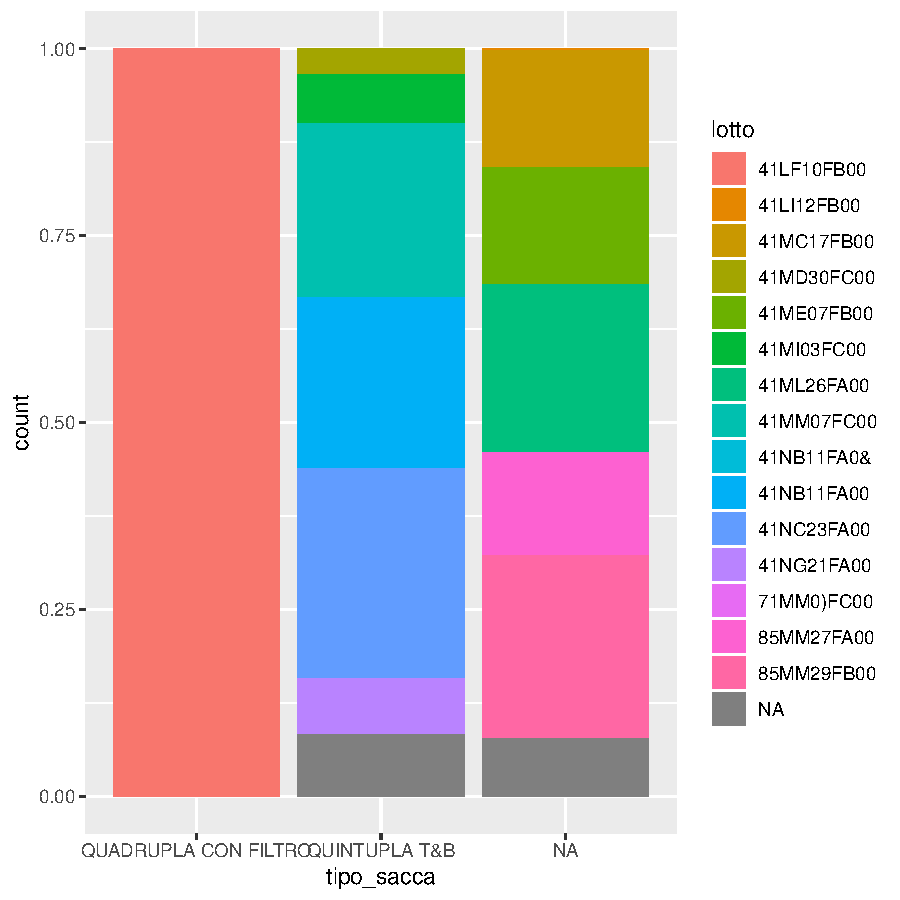
\includegraphics{tidigg-014}
\begin{Schunk}
\begin{Sinput}
> emcxrep00 <- filter(scarico19, cat_emc !="PLT" | descr_reparto != "ESTERNI TERRITORIO")
> emcxrep0 <- filter(emcxrep00, cat_emc != "SIE" & descr_reparto != "KEDRION")
> emcxrep0chi <- filter(emcxrep0, descr_reparto == "PRONTO SOCCORSO MEDICO" | descr_reparto == "ORTOPEDIA I " | descr_reparto == "CH. GENERALE"   | descr_reparto == "UROLOGIA"  | descr_reparto == "CHIRURGIA VASCOLARE"| descr_reparto == "RIANIMAZIONE" | descr_reparto == "OSTETRICIA GINECOLOGIA")
> emcxrep0med<- filter(emcxrep0, descr_reparto != "PRONTO SOCCORSO MEDICO" | descr_reparto != "ORTOPEDIA I " | descr_reparto != "CH. GENERALE"   | descr_reparto != "UROLOGIA"  | descr_reparto != "CHIRURGIA VASCOLARE"| descr_reparto != "RIANIMAZIONE" | descr_reparto != "OSTETRICIA GINECOLOGIA")
> emcxrep <- ggplot(data = emcxrep0) + geom_bar(mapping = aes(x = cat_emc, fill = descr_reparto))
> emcxrepchi <- ggplot(data = emcxrep0chi) + geom_bar(mapping = aes(x = cat_emc, fill = descr_reparto))
> emcxrepmed <- ggplot(data = emcxrep0med) + geom_bar(mapping = aes(x = cat_emc, fill = descr_reparto))
\end{Sinput}
\end{Schunk}

\begin{Schunk}
\begin{Sinput}
> emcxrep + theme(legend.position = "none") +  scale_y_continuous(breaks = seq(500, 4000, by = 500))
\end{Sinput}
\end{Schunk}
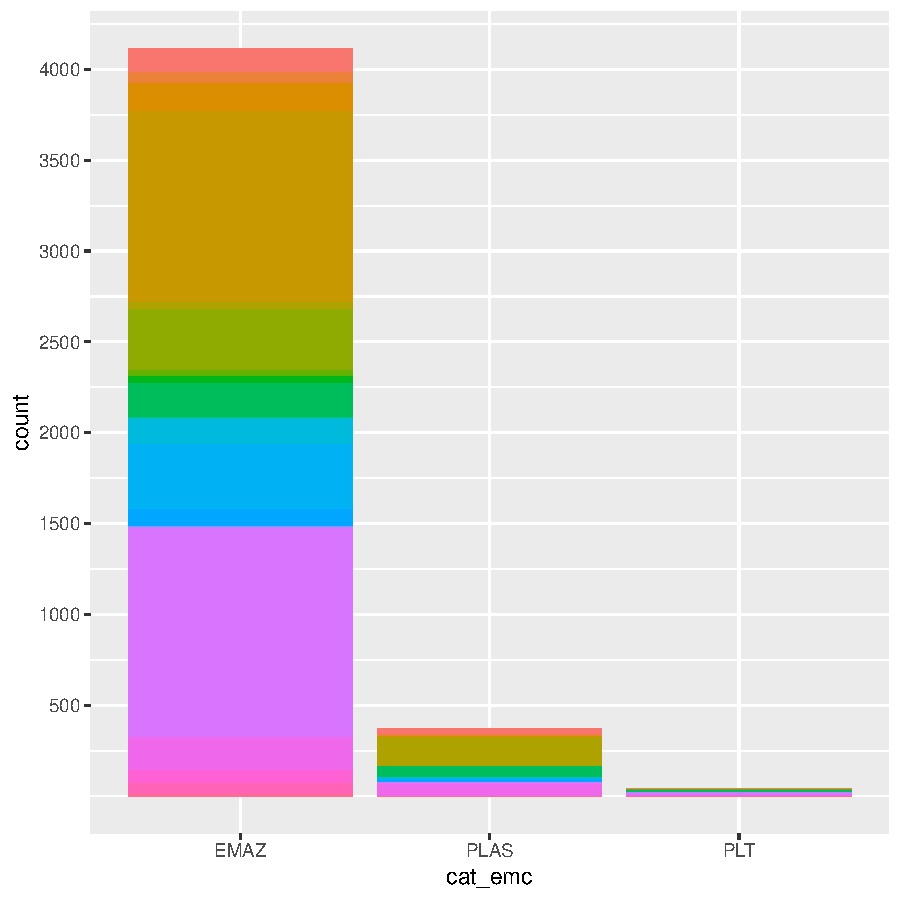
\includegraphics{tidigg-016}
\begin{Schunk}
\begin{Sinput}
> emcxrepchi + theme(legend.position = "bottom") +  scale_y_continuous(breaks = seq(500, 4000, by = 500)) +
+ guides( color = guide_legend( nrow = 3, override.aes = list(size = 2)))
\end{Sinput}
\end{Schunk}
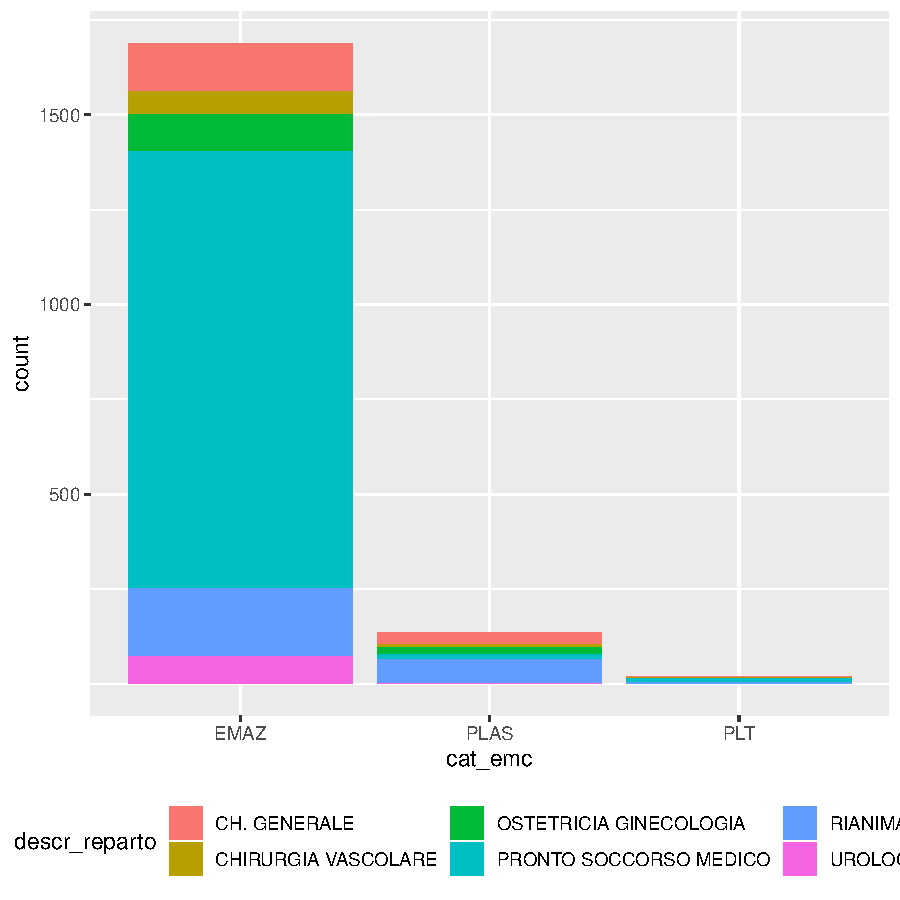
\includegraphics{tidigg-017}
\begin{Schunk}
\begin{Sinput}
> emcxrepmed + theme(legend.position = "bottom") +  scale_y_continuous(breaks = seq(500, 4000, by = 500)) +
+ guides( color = guide_legend (ncol= 2, nrow = 10, override.aes = list(size = 2)))
\end{Sinput}
\end{Schunk}
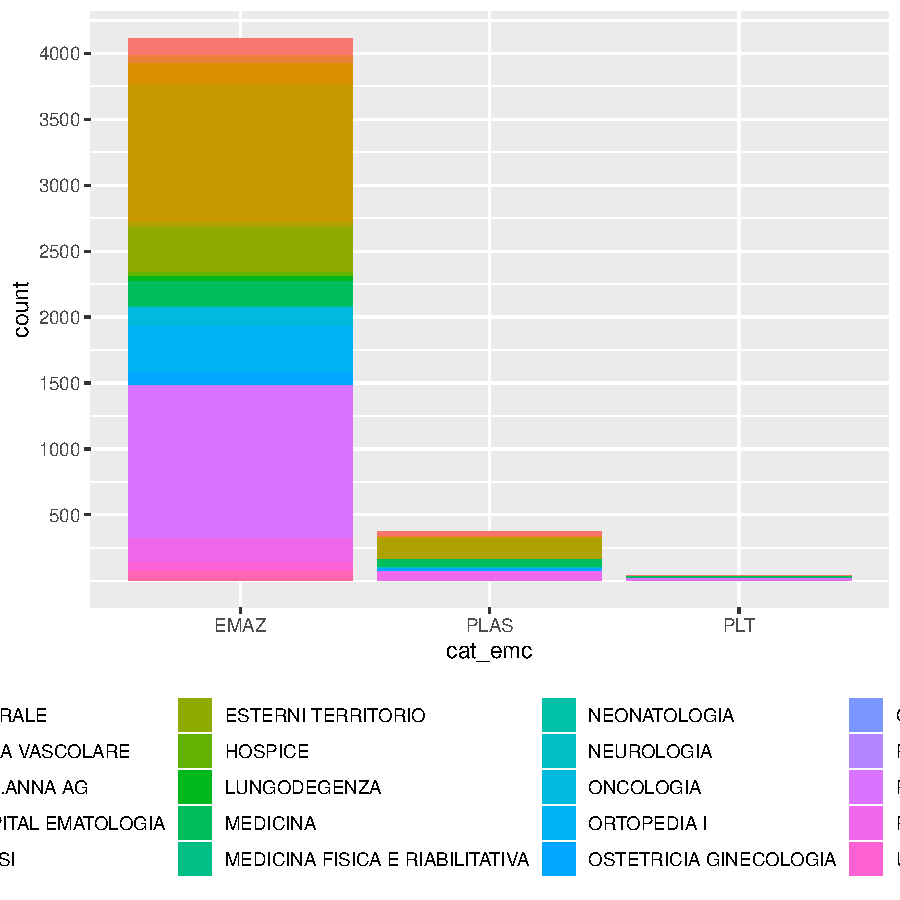
\includegraphics{tidigg-018}

\begin{Schunk}
\begin{Sinput}
> scarico19 %>% filter(descr_reparto=="ORTOPEDIA I") %>% count(codice_anagrafico_individuale)
\end{Sinput}
\begin{Soutput}
# A tibble: 201 x 2
   codice_anagrafico_individuale     n
                           <dbl> <int>
 1                          6034     1
 2                         12792     2
 3                         12964     1
 4                         13446     1
 5                         15901     1
 6                         16296     3
 7                         17259     1
 8                         20201     1
 9                         21610     1
10                         22065     3
# … with 191 more rows
\end{Soutput}
\begin{Sinput}
> scarico19 %>% filter(descr_reparto=="PRONTO SOCCORSO MEDICO") %>% count(codice_anagrafico_individuale)
\end{Sinput}
\begin{Soutput}
# A tibble: 434 x 2
   codice_anagrafico_individuale     n
                           <dbl> <int>
 1                          5847     2
 2                          6530     2
 3                          7464     2
 4                          9723     2
 5                         10704     5
 6                         13737     3
 7                         15480     2
 8                         15482     7
 9                         15784     3
10                         16048     4
# … with 424 more rows
\end{Soutput}
\begin{Sinput}
> 
\end{Sinput}
\end{Schunk}



\begin{Schunk}
\begin{Sinput}
> tapply(scarico19$visualizza_livello, scarico19$descr_reparto, length)
\end{Sinput}
\begin{Soutput}
                   CH. GENERALE             CHIRURGIA VASCOLARE 
                            154                              69 
              CLINICA S.ANNA AG         DAY HOSPITAL EMATOLOGIA 
                            159                            1052 
                     EMODIALISI              ESTERNI TERRITORIO 
                            199                             622 
                        HOSPICE                    LUNGODEGENZA 
                             37                              35 
                       MEDICINA MEDICINA FISICA E RIABILITATIVA 
                            259                               7 
                   NEONATOLOGIA                      NEUROLOGIA 
                              1                               8 
                      ONCOLOGIA                     ORTOPEDIA I 
                            147                             355 
         OSTETRICIA GINECOLOGIA            OTORINOLARINGOIATRIA 
                            117                               2 
                      PEDIATRIA          PRONTO SOCCORSO MEDICO 
                              5                            1178 
                   RIANIMAZIONE                        UROLOGIA 
                            246                              78 
                           UTIC                            UTIN 
                             58                              23 
\end{Soutput}
\begin{Sinput}
> tapply(scarico19$visualizza_livello, scarico19$cat_emc, length)
\end{Sinput}
\begin{Soutput}
EMAZ PLAS  PLT  SIE 
4134 3835  325   13 
\end{Soutput}
\begin{Sinput}
> tapply(scarico19$visualizza_livello, scarico19$cat_emc, length)
\end{Sinput}
\begin{Soutput}
EMAZ PLAS  PLT  SIE 
4134 3835  325   13 
\end{Soutput}
\end{Schunk}
\begin{Schunk}
\begin{Sinput}
> nsaccheperpaz <- tapply(scarico19$codice_anagrafico_individuale, scarico19$descr_reparto, table)
\end{Sinput}
\end{Schunk}


\end{document}
